\documentclass[12pt]{article}

\usepackage{amsmath}
\usepackage[margin = 1in]{geometry}
\usepackage{graphicx}
\usepackage{booktabs}
\usepackage{natbib}
\usepackage{lipsum}
\usepackage{pgfplots}
\pgfplotsset{compat=1.18}
\usepackage{hyperref}
\usepackage{csvsimple}

\title{Assignment 2: Practicing Latex}

\author{Garrick Ho \\
Department of Statistics \\
University of Connecticut}

\begin{document}

\maketitle

\begin{abstract}
This is where the abstract goes.
\end{abstract}

\section{Introduction}
\label{sec:intro}

Use this section to answer three questions:
Why is the topic important/interesting? What has been done on this topic in the literature?
What is your contribution?
\\
The rest of the paper is organized as follows.
The data will be presented in Section~\ref{sec:data}.
The methods are described in Section~\ref{sec:meth}.
The results are reported in Section~\ref{sec:resu}.
A discussion concludes in Section~\ref{sec:disc}.
The appendix is in Section~\ref{sec:appe}.

\section{Data}
\label{sec:data}

Use this section to describe the data that helps to answer your research
questions.

\section{Methods}
\label{sec:meth}

In math, we are able to use \(a^2 + b^2 = c^2\), which is the Pythagorean theorem.\\
\\
Euler's identity is \(e^{i{\pi}} + 1 = 0\).\\
\\
Example of in-display equations:
\\
\begin{equation}
  \label{eq:quad}
  x = \frac{-b \pm \sqrt{b^2 - 4ac}}{2a}
\end{equation}
\\
\begin{equation}
  \label{eq:pois}
  f(x) = \frac{\lambda^2}{x!}e^{-\lambda}
\end{equation}
\\
Equation~\ref{eq:quad} is the quadratic formula.\\
\\
Equation~\ref{eq:pois} is the Poisson distribution.

\section{Results}
\label{sec:resu}



\section{Discussion}
\label{sec:disc}

Table and plot from the Airquality dataset from R:

\begin{table}[htbp]
    \centering
    \csvautotabular{airquality_table.csv}
    \caption{Table}
    \label{tab:airquality_table}
\end{table}

\begin{figure}[htbp]
    \centering
    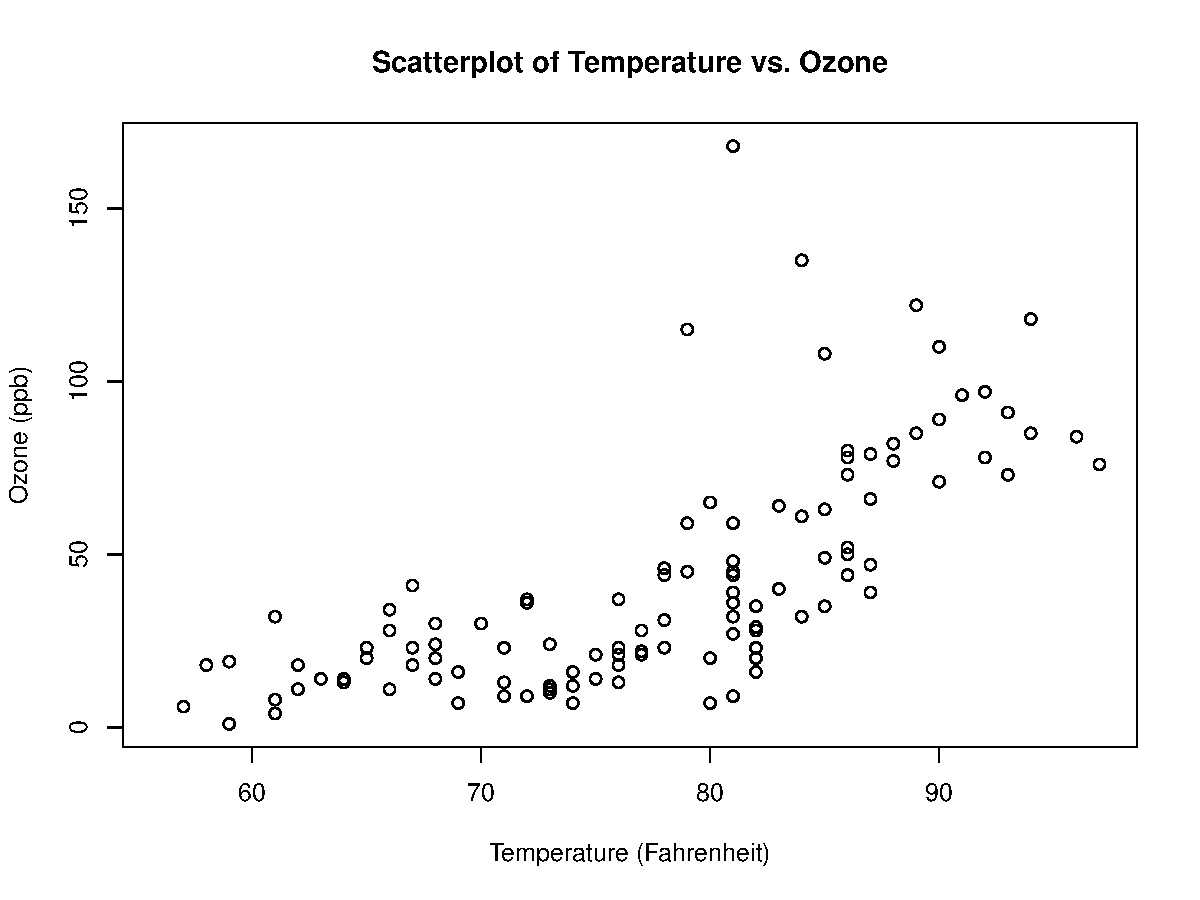
\includegraphics[width=.8\textwidth]{airquality_plot.pdf}
    \caption{Scatterplot}
    \label{fig:airquality_plot}
\end{figure}

In Figure \ref{fig:airquality_plot}, we can see that there is a positive association between Ozone and Temperature.
\\
In table \ref{tab:airquality_table}, we can see that there are some missing values in the table. 

\section{Appendix}
\label{sec:appe}

This is a textual citation of \citet{Fan2014}.\\
This is a parenthetical citation of Thomas Davenport's report \citep{Davenport2012}.

\bibliographystyle{plainnat}
\bibliography{refer}
\end{document}